\section{Description}

The gamma distribution was created to predict the wait time until future events. While the exponential distribution
predicts the wait time until the \textbf{first} event happens, the gamma distribution predicts the wait time until the
\textbf{\textit{k}th} event occurs.

% TODO
TODO: https://towardsdatascience.com/gamma-distribution-intuition-derivation-and-examples-55f407423840

We represent the gamma distribution by $\gamma(p, \alpha)$.

\subsection{Probability density function}
For $\alpha > 0$ and $p > 0$:
\[
	f(x) = \frac{\alpha^p}{\Gamma(p)} x^{p - 1} e^{-\alpha x}, \text{ for } x > 0
\]

Note that $f(x) > 0$ for $x > 0$, and:
\[
	\int_0^\infty f(x) \, dx = \frac{1}{\Gamma(p)} \int_0^\infty y^{p - 1} e^{-y} \, dy= 1
\]
because the definition of $\Gamma(p)$ is the value of the last integral.

\begin{figure}[H]
	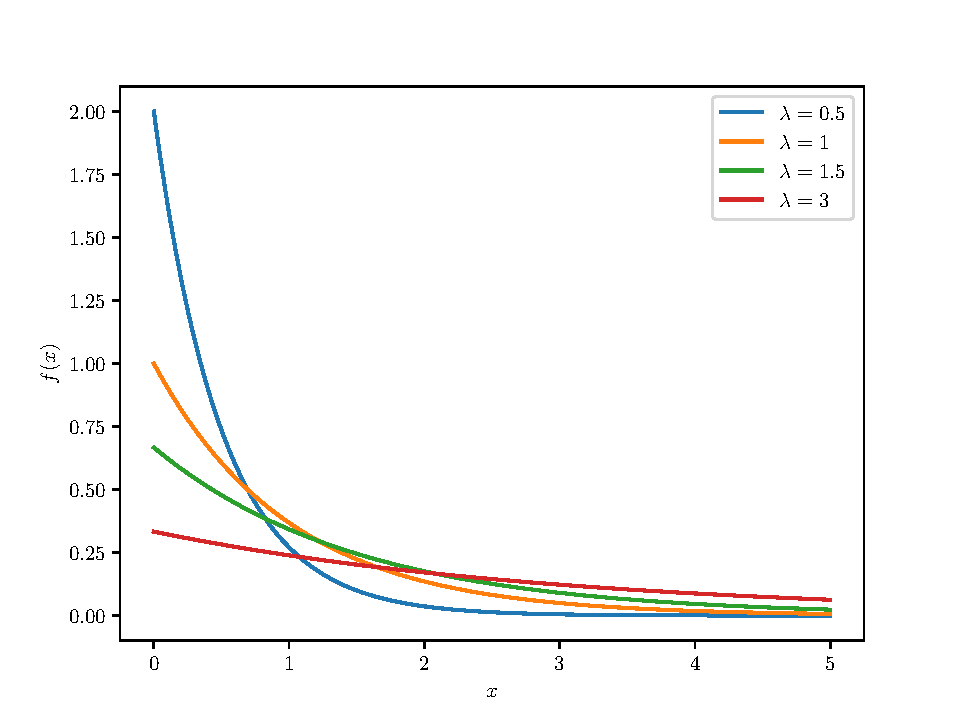
\includegraphics[width=\textwidth]{r/gamma/pdf.pdf}
	\caption{$f(x) = \frac{\alpha^p}{\Gamma(p)} x^{p - 1} e^{-\alpha x}, \text{ for } x > 0$, pdf of $\gamma(p, \alpha)$}
\end{figure}


\subsection{Cumulative distribution function}
For $\alpha > 0$ and $p > 0$:
\[
	F(x) = \int_0^x \frac{\alpha^p}{\Gamma(p)} t^{p - 1} e^{-\alpha t} \, dt \text{, for } x > 0
\]

$F$ can't be expressed in terms of elementary functions, but its values can be calculated.

\begin{figure}[H]
	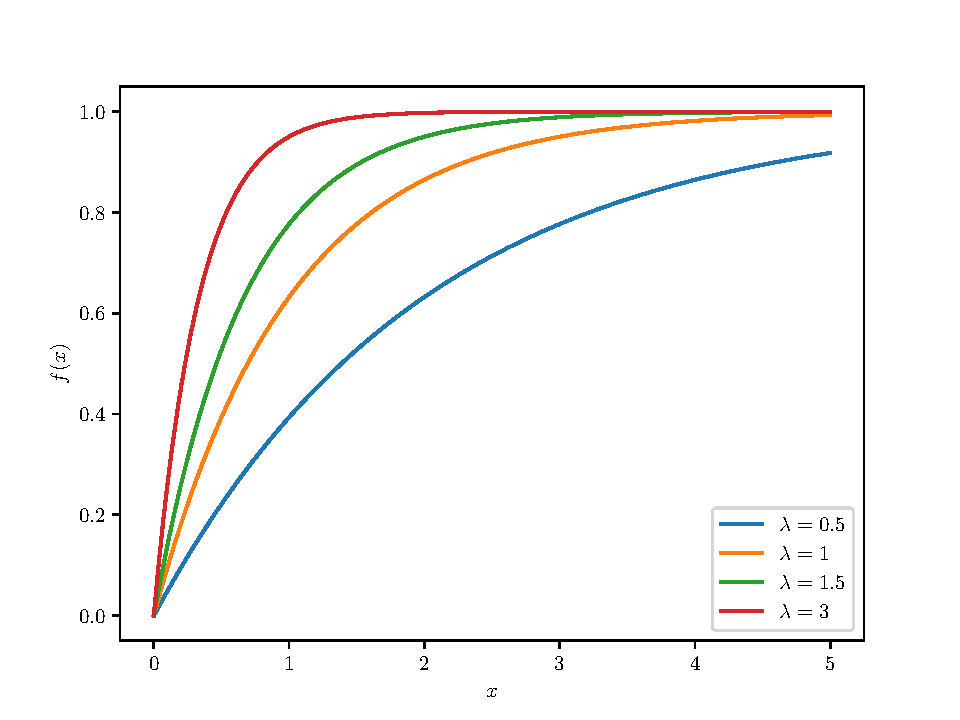
\includegraphics[width=\textwidth]{r/exponential/cdf.pdf}
	\caption{$F(x) = \int_0^x \frac{\alpha^p}{\Gamma(p)} t^{p - 1} e^{-\alpha t} \, dt \text{, for } x > 0$, cdf of $\gamma(p, \alpha)$}
\end{figure}

\section{Properties}
\begin{itemize}
	\item For $p = 1$, the Gamma distribution is the same as the exponential one.
	\item For $p < 1$, the density of Gamma distribution is unbounded when $x \rightarrow 0^+$, so the formula is an improper integral (which converges).
	\item For $p > 1$, the density function tends to 0 as $x \rightarrow 0^+$.
\end{itemize}

The parameter $p$ determines the shape of the density function. The parameter $\alpha$, however, is a scale parameter which expands or contracts the x axis. Indeed, if we use the change of variables $y = x/a$, with $a > 0$, we see that:
\[
	\frac{\alpha^p}{\Gamma(p)} x^{p - 1} e^{-\alpha x} \, dx \ \text{ turns into } \
	\frac{(a\alpha)^p}{\Gamma(p)} y^{p - 1} e^{-\alpha a y} \, dy
\]
so that the probability that $\gamma(p, \alpha)$ assigns to the neighborhood of a point $x$ is the same that $\gamma(p, \alpha a)$ assigns to the neighborhood of the point $y = x/a$.
In particular, if $a = 1/\alpha$, the distribution $\gamma(p, \alpha)$ becomes $\gamma(p, 1)$ with the change of variables $y = \alpha x$.

\section{Moments}

\begin{tabularx}{\textwidth}{s X}
	\hline
	Mean & ?? \\\hline
	Variance & ?? \\\hline
\end{tabularx}


